%!TEX program = xelatex

\documentclass[12pt]{article}
\usepackage[utf8]{inputenc}
\usepackage[a4paper]{geometry}
\usepackage[dvipsnames]{xcolor} %paquete para manejar colores
\usepackage[colorlinks=true, linkcolor=cyan]{hyperref}
\usepackage{tocloft} %Paquete que añade puntos sucesivos
\usepackage{amssymb} %Para formulas y simbología matemática
\usepackage{mathrsfs}%para las cursivas matematicas
\usepackage{amsthm}%para los postulados
\usepackage{amsmath}%Para más formulas 
\usepackage{multirow}%Crea celdas que ocupan multiples filas
%para dibujo chulo
\usepackage{adjustbox}
\usepackage{tikz}
\graphicspath{images}
\usepackage{lineno}
\usepackage{ragged2e}
\usepackage[rightcaption]{sidecap}
\usepackage{lipsum}
\usepackage{framed}
\usepackage{graphicx}
\usepackage{subcaption}
\usepackage{afterpage}
\usepackage{fancyhdr}
\usepackage{fancyvrb}
\usepackage{fontspec}
\usepackage{float}
\usepackage{booktabs}
\usepackage{siunitx}
\usepackage[
backend=biber,
style=phys,
biblabel=brackets,
sorting=none
]{biblatex}
\addbibresource{referencias.bib} 
\usepackage{wrapfig}%Para introducir tablas o figuras en medio del texto
\usetikzlibrary{positioning, arrows.meta} %libreria que permite hacer gráficas guays utilizando below=of
\numberwithin{equation}{section}%para que las formulas se nombren de acuerdo a la sección
\renewcommand{\figurename}{Figura}
\renewcommand{\tablename}{Tabla}


%con esto se renombran las figuras
\renewcommand{\thefigure}{\arabic{section}.\arabic{figure}}

%\bibliographystyle{plain}%en teoria esto sirve para ordenar las bibliografias por orden de nombramiento

\renewcommand{\contentsname}{Índice}

% Configuración del formato del índice

\renewcommand{\cftsubsecleader}{\cftdotfill{\cftdotsep}} % Puntos líderes para subsecciones
\cftsetindents{section}{0em}{2em}  % Ajusta la indentación de las secciones en el índice
\cftsetindents{subsection}{2em}{3em}  % Ajusta la indentación de las subsecciones en el índice

% Configuración de colores para los enlaces
\hypersetup{
    colorlinks=true,
    linkcolor=blue,     % Color de los enlaces internos (secciones, subsecciones)
    filecolor=magenta,  % Color de los enlaces a archivos
    urlcolor=cyan,      % Color de los enlaces a URLs
}



%%%%%%%%%%%% LETRAREN ITURRIA ALDATZEKO (EHUSans) %%%%%%%%%%%%
\setmainfont{EHUSans-Light.otf}[ % Nombre completo del archivo Regular
  Path = ./EHU Sans/,                        % Cambia esto si las fuentes están en una subcarpeta
  BoldFont = EHUSans-Regular,     % Nombre completo del archivo Bold
  ItalicFont = EHUSans-Italic, % Nombre completo del archivo Italic
  BoldItalicFont = EHUSans-BoldItalic, % Nombre completo del archivo BoldItalic
]
\newfontface\lightfont{EHUSans-Light.otf}[Path=./EHU Sans/]
\newfontface\blackfont{EHUSans-Black.otf}[Path=./EHU Sans/]

%%%%%%%%%%%%%%%%%%%%%%%%%%%%%%%%%%%%%%%%%%%%%%%%%%%%%%%%%%%%%%%%%


\geometry{top=2.5cm, bottom=2.5cm, left=2.5cm, right=2.5cm}
\begin{document}

\definecolor{light-gray}{gray}{0.87}  

\begin{titlepage}
\hspace*{-3.5cm}
    \begin{minipage}{\textwidth}
        \vspace{-2.5cm}
        \begin{center}
            \includegraphics[width=\paperwidth]{TFG_portada-Latex/LogoEHU.PNG}
        \end{center}
    \end{minipage}

\vspace{1cm}

\hspace{-3.1cm}
\noindent\fcolorbox {light-gray}{white}{

    \parbox{\paperwidth}{
     \begin{center}
     \large Trabajo fin de grado
    \\
             \large Grado en Física

\end{center}
    }
    }


\vspace{0.8cm}

\noindent\hspace*{-2.5cm}%
\colorbox{light-gray}{\begin{minipage}{\paperwidth}%

    \vspace{1cm}

    \color{RoyalBlue}
    \centering\Large\textbf{ Desarrollo de un algoritmo para la calibración de la distorsión óptica en adquisión de imágenes satelitales y comprobación experimental
}
    \\
    \centering\textmd{ Lanaren azpitituloa / Subtitulo del trabajo}


    \vspace{7.5cm}\mbox{}
  \end{minipage}
}

\begin{flushright}
 Egilea/ Autor/a:
\\
Xabier Joel Yoldi García
\\
Zuzendariak/Directores/as:
\\
Josu Mirena Igartua Aldamiz
\\
Iñigo Irizar Loibide        
\\
\end{flushright}

\begin{center}
\noindent\fcolorbox {white}{white}{

    \parbox{11cm}{
         \begin{center}
    \footnotesize © 2021, se puede proteger poniendo nombre y apellido/izen abizenak ezarriz babes zaitezke edo lizentzia CC batekin babestu / o con una licencia CC
    \\
   \small http://es.creativecommons.org/blog/licencias/

        \end{center}
    }
    }
\end{center}

\hspace{-3.2cm}
\noindent\fcolorbox {light-gray}{white}{
    \begin{minipage}[]{1000pt}

        \parbox{\paperwidth}{
            \begin{center}
    
                 Leioa, 2025eko maiatzaren 12a / Leioa, 12 de Mayo de 2025

            \end{center}
        }
    \end{minipage}
}
\end{titlepage}


%%%%%%%%%%%%%%%%%%%%%%%%%%%%%%%
%Hemendik aurrera hasi lana idazten%
%%%%%%%%%%%%%%%%%%%%%%%%%%%

\pagestyle{fancy}
% Elimina la línea horizontal en la parte superior del encabezado
%\renewcommand{\headrulewidth}{0pt}

% Configura el contenido del encabezado
\fancyhead[R]{X. J. Yoldi García}
\fancyhead[L]{\nouppercase{\leftmark}}
\tableofcontents
\newpage

\section{Introducción}

La industria aeroespacial y de observación terrestre ha crecido en los últimos años ampliamente y cada vez demanda sistemas más precisos debido a la carrera tecnológica que existe. En este contexto, la empresa Satlantis Microsats se ha especializado en el desarrollo de cámaras de alta resolución para pequeños satélites (microsatélites). Para garantizar la calidad y la fiabilidad de las imágenes capturadas, es esencial el desarrollo de sistemas con una calidad excelente y una mecánica cuidada al detalle. Sin  embargo, es fundamental procesar las imágenes para caracterizar y corregir las posibles aberraciones ópticas que pudieran tener los sistemas de captura. Este campo, denominado comúnmente como \textit{Image Proccessing}, es el encargado de realizar dichas correcciones, así como de aumentar la calidad de las imágenes o caracterizar patrones para futuras aplicaciones \textit{(en Satlantis la detección de metano es un proyecto en curso)}.\\

En la actualidad, una aberración presente en todos los sistemas ópticos es la distorsión óptica. Esta aberración es producida por la forma esférica característica de muchas lentes y provoca un ligero desplazamiento en las posiciones de la imagen. Principalmente, existen dos formas en las que se distorsionan las capturas, denominadas tipo barril o cojín. Debido a la gran sensibilidad que existe para caracterizar esta aberración, la forma más sencilla y utilizada para abordar este problema es corregirla en base a medidas experimentales de cada sistema. Es por ello que en este Trabajo de Fin de Grado se desarrolla una metodología para la medida y análisis de la distorsión óptica con el objetivo final de aplicarlas en las cámaras de Satlantis.\\

Para ello se ha empleado un banco de ensayo experimental que consiste en una placa de pinholes (orificios del orden de los micrómetros), que, al alumbrarlos, actúan como fuentes puntuales de luz. Las fotografías tomadas de dicha placa permiten, mediante técnicas desarrolladas en este Trabajo de Fin de Grado, medir los desplazamientos relativos de cada punto y así calcular el perfil de distorsión introducido por la lente.\\

Como fase preliminar y para realizar una validación de la metodología, se ha elaborado una etapa de simulaciones. En esta etapa se han generado imágenes replicando las imágenes proporcionadas por Satlantis, y se les ha aplicado una distorsión artificial. Esto ha permitido desarrollar y ajustar los algoritmos de detección y medición del perfil de distorsión.\\

La memoria se estructura en los siguientes apartados: en primer lugar, se explica el marco teórico y el fenómeno de distorsión óptica y como modelarlo matemáticamente. A continuación, se desarrolla la metodología propuesta para la detección de distorsión y se valida y valora con diferentes simulaciones. Finalmente, se presentan los resultados obtenidos con las imágenes de Satlantis y se concluye con una valoración del método propuesto.

\newpage
\section{Sistemas Electro-Ópticos}
\label{sec: Sistemas Electro-Ópticos}
Los sistemas ópticos conforman un campo muy interesante en el contexto científico debido a la variedad de sistemas que podemos encontrar. Desde un ojo humano hasta una cámara o, incluso, un telescopio son parte de este área. Sin embargo, cuando se desea caracterizar un sistema óptico en concreto, una medida comúnmente utilizada es la Función de Dispersión de Punto (PSF), que es una función en el dominio espacial. En concreto, se utiliza su función análoga en el espacio de frecuencias, la Función de Transferencia Óptica (OTF), que no es más que su transformada de Fourier bidimensional. Esta función da cuenta de la respuesta a una señal sinusoidal periódica a través de los diferentes componentes del sistema óptico, en función de su frecuencia espacial \cite{williamsOTF}. 

\begin{equation}
    OTF = F[PSF]
\end{equation}

La principal ventaja de trabajar con la OTF radica en la facilidad que muestra para estudiar el comportamiento de un sistema donde varios subsistemas están combinados. Esto es porque la función de transferencia de todo el sistema óptico puede expresarse como multiplicación de la función de transferencia de cada subsistema individual. Además, es de gran utilidad para detectar e implementar mejoras en cada subsistema.\\

No obstante, la calidad de la OTF y, en consecuencia, del sistema óptico, también depende de los componentes electrónicos que lo conforman. Los principales elementos que afectan a la OTF son los píxeles que conforman el sensor óptico y el ruido electrónico (que afecta a todos los aparatos electrónicos). Por lo tanto, es necesario saber cómo el tamaño del píxel afecta a la OTF de todo el sistema electro-óptico.\\

\subsection{Sistemas Ópticos}

\subsubsection{Respuesta al impulso}

La respuesta al impulso \(h(x, y)\) o PSF, describe la respuesta de un sistema de imágenes a una fuente puntual o un objeto puntual. Esta función viene descrita por la anchura de la respuesta al impulso y, en esencia, es el resultado de la combinación de aberraciones y efectos de difracción, inherentes a los sistemas ópticos.\\

Comúnmente, la PSF es interpretada como la distribución del brillo en función de la posición. En sistemas ópticos incoherentes, si se capturan dos objetos diferentes al mismo tiempo, la imagen de cada objeto no se ve afectada por el otro, debido a la propiedad no interactuante de los fotones. Esto significa que la imagen resultante \( g(x, y) \) se puede expresar como la imagen ideal \( f(x, y) \) convolucionada (\(\ast\)) con la respuesta al impulso \( h(x, y) \).
 
\begin{equation}
    g(x, y) = f(x, y) \ast h(x, y)
    \label{eq: convolucion}
\end{equation}

\newpage
\textit{Prueba:}\\

Considerando una situación unidimensional, la señal de entrada \( f(x) \) es analizada por el sistema óptico (lineal e invariante) aplicando la transformación \( T \) a la señal de entrada, y este sistema devuelve la señal de salida \( g(x) \).

\begin{equation*}
    g(x) = T[f(x)]
\end{equation*}

Esto se puede escribir de la siguiente manera usando la función Delta:

\begin{equation*}
    g(x) = T \left[ \int_{-\infty}^{\infty} f(\tau) \delta(x - \tau) d\tau \right]
\end{equation*}

Dado que el sistema óptico es lineal,

\begin{equation*}
    g(x) = \int_{-\infty}^{\infty} f(\tau) T[\delta(x - \tau)] d\tau
\end{equation*}

La respuesta al impulso se define como la respuesta del sistema óptico a una fuente puntual, idealmente una función Delta:

\begin{equation*}
    h(x) = T[\delta(x)]
\end{equation*}

Entonces, debido a que el sistema óptico también es invariante,

\begin{equation*}
g(x) = \int_{-\infty}^{\infty} f(\tau) h(x - \tau) d\tau
\end{equation*}

Esta última ecuación es precisamente la definición matemática de convolución.

\begin{equation*}
g(x) = f(x) * h(x)
\end{equation*}

Este cálculo se puede extrapolar a una situación bidimensional, obteniendo un resultado análogo a la Ecuación~\ref{eq: convolucion}.

\begin{equation*}
g(x, y) = f(x, y) * h(x, y)
\end{equation*}

De este resultado se puede derivar lo siguiente: si el sistema tuviera una resolución y calidad perfectas, la respuesta del sistema coincidiría con la imagen ideal. Atendiendo a la Ecuación~\ref{eq: convolucion}, esto es lo mismo que afirmar que la respuesta del sistema \(h(x, y)\) es una función delta. Lo que concluye en la idea de que la PSF da cuenta de la calidad de la imagen en función de su ancho espacial: cuanto más estrecha es la PSF, mejor es la imagen final.\\ 


\begin{figure}[h!]
\centering
\includegraphics[width=0.5\textwidth]{Imagenes/convolucion.png}
\caption{\small Ilustración mostrando la imagen ideal de dos puntos brillantes, la PSF del sistema óptico y la imagen resultante obtenida al hacer la convolución de los dos primeros.}
\label{fig:PSF}
\end{figure}

\subsubsection{Dominio de frecuencias}

Como bien se ha comentado anteriormente, la PSF y OTF son funciones análogas en distintos dominios. En esta sección se aborda el proceso de obtención de imágenes desde la perspectiva frecuencial, es decir, estudiando la OTF en vez de la PSF.\\

Según el teorema de la convolución, una convolución en el dominio espacial es igual a una multiplicación en el dominio de frecuencia. De este modo, al aplicar una transformada de Fourier en ambos lados de la Ecuación~\ref{eq: convolucion} se obtien la siguiente expresión:

\begin{equation}
\mathcal{F}[g(x, y)] = \mathcal{F}[f(x, y) * h(x, y)]
\end{equation}

Se pueden definir las siguientes funciones en el dominio de frecuencia:

\begin{equation}
G(\xi, \eta) = F(\xi, \eta) \cdot H(\xi, \eta)
\end{equation}

donde $\xi = 1/X$ y $\eta = 1/Y$, suponiendo que $X$ y $Y$ son los períodos de las señales sinusoidales en $x$ e $y$. $H(\xi, \eta)$ es la respuesta del sistema óptico a una fuente puntual en el dominio de frecuencias, es decir, la OTF, que se expresa como $H(\xi, \eta) = OTF(\xi, \eta)$.\\

Si se analiza un sistema óptico compuesto por \(N\) subsistemas, la respuesta del sistema al completo será la multiplicación de la imagen ideal \(F(\xi, \mu)\) y la respuesta individual de cada subsistema \(H_i(\xi, \mu)\).

\begin{equation}
G(\xi, \eta) = F(\xi, \eta) \cdot \prod_{i=1}^NH_i(\xi, \mu)
\end{equation}

Por lo que, la multiplicación de todas las respuestas individuales de cada subsistema \(H_i(\xi, \mu)\), se puede interpretar como la respuesta del sistema total.\\

\begin{equation*}
    H(\xi, \mu) = \prod_{i=1}^NH_i(\xi, \mu)
\end{equation*}

Comúnmente, esta función es compleja y se puede describir como la multiplicación de su módulo y su fase. En óptica, el módulo se conoce como Función de Transferencia de Modulación (MTF) y la fase como Función de Transferencia de Fase (PTF).

\newpage
\begin{equation}
    OTF = H(\xi, \eta) = |H(\xi, \eta)| e^{i\theta(\xi, \eta)}
\end{equation}

donde

\begin{equation*}
    MTF = |H(\xi, \eta)| \quad ; \quad PTF = \theta(\xi, \eta)
\end{equation*}

Como consecuencia de las propiedades de las transformadas de Fourier, el hecho de tener una PSF simétrica \(h(\xi, \mu) = h(-\xi, -\mu)\), hace que su transformada (OTF) sea una función real pura \cite{bracewell2000}. En otras palabras, una PSF simétrica implica una OTF igual a la MTF y una PTF nula.\\

Como bien se acaba de introducir, la MTF se define como el módulo de la OTF. En concreto, la MTF es la función que define la capacidad de resolución del sistema óptico. Es decir, con esta herramienta se mide la efectividad que tiene el sistema para representar el contraste de la imagen original a diferentes frecuencias. De esta forma se define la cantidad \(M\) (en inglés \textit{modulation depth}) como:

\begin{equation}
    M = \frac{A_{max}-A_{min}}{A_{max}+A_{min}}
\end{equation}

donde \(A_{max}\) y  \(A_{min}\) son la irradiación máxima y mínima a contrastar.\\

Por su definición, la MTF incluye todos los posibles efectos de cualquier imperfección que contribuye a la degradación de la imagen, como la difracción, aberraciones cromáticas, distorsión, etc. Una posible consecuencia directa de estas imperfecciones es la pérdida en la simetría de la PSF. Cuando esto ocurre, la PTF ya no es nula y se vuelve más significativa. Por esta razón, la PTF se utiliza comúnmente para analizar la presencia e importancia de esas imperfecciones.\\

\begin{figure}[h]
    \centering
    \includegraphics[width=0.75\linewidth]{Imagenes/contraste.png}
    \caption{\small Comparación del contraste en los planos objeto e imagen.\cite{EdmundOpticsMTF}}
    \label{fig: contraste}
\end{figure}

En la siguiente sección se dará una introducción a diferentes fuentes que dan lugar a estas imperfecciones. En concreto, se estudiará la distorsión óptica, que es la aberración causa de este trabajo. 

\subsection{Fuentes de degradación en la calidad de la imagen}

Como bien se ha comentado, los sistemas ópticos cuentan con multitud de imperfecciones que afectan a la formación de imágenes. Dos grandes causas de una mala formación en las imágenes son las aberraciones ópticas y el ruido electrónico que, como se ha comentado en la Sección\ \ref{sec: Sistemas Electro-Ópticos} afecta a la OTF.\\

\subsubsection{Aberraciones ópticas}
Las aberraciones ópticas son desviaciones de la propagación ideal de los rayos de luz a través de un sistema óptico. Estas desviaciones provocan que los rayos no converjan adecuadamente, provocando errores en la imagen. Las aberraciones se clasifican comúnmente en dos grandes grupos: aberraciones monocromáticas y aberraciones cromáticas. La principal diferencia entre ambas es la respuesta que tienen a diferentes colores. 

Las aberraciones monocromáticas aparecen incluso si la luz utilizada es de un solo color (longitud de onda fija) y son principalmente las siguientes:

\begin{itemize}
\item \textbf{Aberración esférica}: Se produce cuando los rayos incidentes alejados del eje óptico se enfocan en diferentes puntos que los rayos cercanos al eje.
\item \textbf{Coma}: Afecta a los rayos que inciden oblicuamente al sistema óptico, generando imágenes de puntos como manchas asimétricas.
\item \textbf{Astigmatismo}: Provoca que los rayos en diferentes planos focales tengan distintos puntos de enfoque.
\item \textbf{Curvatura de campo}: Hace que una imagen plana se proyecte en una superficie curva.
\item \textbf{Distorsión}: Provoca un desplazamiento de las posiciones de los puntos de la imagen respecto a su posición ideal, sin afectar la nitidez.
\end{itemize}

En cambio, las cromáticas se originan debido a que el índice de refracción de los materiales ópticos depende de la longitud de onda de la luz. Los rayos de diferentes colores se enfocan en distintos puntos, dando lugar a halos o bordes coloreados en las imágenes.

\subsubsection{Relación señal a ruido (SNR)}
\label{sec:ruido}
Hay tres fuentes principales de ruido que afectan a los sistemas electro-ópticos: corriente oscura, ruido de disparo y ruido de lectura.

\begin{itemize}
    \item \textbf{Corriente oscura:} Es el efecto de la corriente eléctrica relativamente pequeña que fluye a través de dispositivos fotosensibles como los sensores, incluso cuando no entran fotones en el dispositivo. Físicamente, la corriente oscura es debida a la generación aleatoria de electrones y huecos dentro de la región de agotamiento del dispositivo. Estos pares electrón-hueco se generan por energía térmica, por lo que este ruido está directamente relacionado con la temperatura. Cuanto mayor es la temperatura a la que trabaja el detector, mayor será este ruido. Además, este ruido depende del tiempo de exposición, ya que se generarán más electrones cuanto más tiempo dure el uso. Se puede corregir restando a la imagen un fotograma (incluso se podría mejorar haciéndolo con la media de muchos) oscuro, denominado \textit{Dark Frame}.
    
    \item \textbf{Ruido de disparo:} El ruido de disparo existe porque fenómenos como la luz y la corriente eléctrica consisten en el movimiento de paquetes discretos. Las fluctuaciones en la corriente de luz que se dan por la cuantización de la luz son la causa de este tipo de ruido. Con un ejemplo se entiende mejor. Un sensor es golpeado por una intensidad lumínica \(I\), esto quiere decir que, de media, en un segundo golpearán un número de fotones proporcionales a \(I\). Sin embargo, dependiendo del tiempo de exposición de la imagen y más variables aleatorias, la cantidad de fotones que recibe el sensor es \textit{pseudo-aleatoria}, dano lugar a deteecciones parásitas que son más significativas a bajas intensidades (por ejemplo al obtener una \textit{Dark Frame}). Estas fluctuaciones siguen una distibución de Poisson. 
    \begin{equation}
        P[X=k] = \frac{e^{-S}S^k}{k!}
    \end{equation}
    donde \(k=0, 1, 2, \dots\) es el número de fotones que golpean el sensor en un intervalo de tiempo concreto. La cantidad \(S\) se puede entender como el número de fotones por unidad de área y unidad de tiempo (en este contexto por \(\mu\text{\small m}^2\) por segundo). Normalmente, esto es interpretado como la "señal".

    \item \textbf{Ruido de lectura:} Es una combinación de ruido proveniente del píxel y del Convertidor Analógico a Digital (ADC). El Ruido de Lectura (RN) del sensor es el nivel equivalente de ruido en la salida de la cámara en oscuridad y con tiempo de integración cero, o dicho de otro modo, el ruido generado al convertir la señal de analógico a digital. Este tipo de ruido no depende del tiempo de exposición ni de la irradiancia, como los otros dos. El ruido de lectura básicamente determina la resolución del contraste que la cámara puede alcanzar. Cuanto menor es el nivel de ruido de lectura, menor es el número mínimo de electrones de señal que se pueden detectar. Un menor ruido de lectura significa que pueden detectarse cambios más pequeños en la amplitud de la señal, y por tanto, se detectan detalles con diferencias de contraste más pequeñas. Este ruido sigue una distribución normal,
    \begin{equation}
        N(\mu, \sigma^2) = \frac{1}{\sigma\sqrt{2\pi}}e^{-\frac{1}{2}(\frac{x-\mu}{\sigma})^2}
    \end{equation}
    donde \(\mu\) es la media y \(\sigma\) la desviación estándar de la señal.\\
\end{itemize}


Como los diferentes ruidos no están correlacionados, el ruido total será simplemente la suma de todos ellos. Pero, evidentemente, todo el ruido descrito ahora, depende de la señal de entrada. Para cuantificar la relación entre la señal de entrada y el ruido generado se define la Relación señal a ruido (SNR). Esta cantidad cuenta la relación entre la potencia de la señal y del ruido.
\begin{equation}
    SNR=\frac{P_{signal}}{P_{noise}}
    \label{eq:SNR}
\end{equation}

Esta SNR varía dependiendo de la señal, y por lo tanto, en una sola imagen, pueden existir múltiples valores de SNR, principalmente porque depende de la reflectividad de la superficie del objeto. Por eso, es difícil definir la SNR de una sola imagen.

\subsubsection{Distorsión Óptica}

La distorsión óptica altera la posición de los puntos de la imagen. Dada  la geometría esférica de las lentes, la distorsión es, a grandes rasgos, una aberración radial. Es decir, la desviación de la posición ideal de los puntos depende de la distancia a la que se encuentren del centro de distorsión. A diferencia de otras aberraciones, no degrada directamente la nitidez de la imagen, pero sí modifica su forma. De forma general, se pueden diferenciar dos tipos de distorsión radial que corresponden a un modelado matemático análogo (en la siguiente sección se explica más en detalle): \textit{pincushion} y \textit{barrel}. 

\begin{figure}[htbp]
    \centering
    \begin{minipage}{\textwidth}
        \centering
        % Subfigura 1
        \begin{subfigure}[b]{0.31\textwidth}
            \includegraphics[width=\linewidth]{Imagenes/imagen_original.jpg}
            \caption{\small Imagen original\\sin distorsión}
            \label{fig:original}
        \end{subfigure}
        \hfill
        % Subfigura 2
        \begin{subfigure}[b]{0.31\textwidth}
            \includegraphics[width=\linewidth]{Imagenes/imagen_distorsionada_pincushion.png}
            \caption{\small Distorsión\\\textit{pincushion}}
            \label{fig:pincushion}
        \end{subfigure}
        \hfill
        % Subfigura 3
        \begin{subfigure}[b]{0.31\textwidth}
            \includegraphics[width=\linewidth]{Imagenes/imagen_distorsionada_barrel.png}
            \caption{\small Distorsión\\\textit{barrel}}
            \label{fig:barrel}
        \end{subfigure}
    \end{minipage}
    \caption{Comparación de los efectos de distorsión óptica}
    \label{fig:distorsiones}
\end{figure}

\subsubsection{Modelado Matemático}

En la actualidad, existen dos modelos dominantes en el contexto científico. El primero es el polinomio propuesto por Duane \cite{Duane} que expresa la posición real (distorsionada) de cada punto \(X=(x, y)\) de la siguiente forma: 
\begin{equation}
\left\{
\begin{aligned}
x = (1 + k_1 ||p||^2 + k_2 ||p||^4 + k_3 ||p||^6 + \dots) u\\
y = (1 + k_1 ||p||^2 + k_2 ||p||^4 + k_3 ||p||^6 + \dots) v 
\end{aligned}
\right.
\label{eq: Duane}
\end{equation}

donde \(k_1, k_2, k_3, \dots\) son los parámetros de distorsión radial (o coeficientes) y \(p=(u,v)\) son las coordenadas de píxel (ideales, sin distorsión) relativas al centro de distorsión del sistema. El otro modelo es una división propuesta por Fitzgibbon \cite{Fitzgibbon}:
\begin{equation}
\left\{
\begin{aligned}
u = \frac{1}{(1 + \lambda_1 ||X||^2 + \lambda_2 ||X||^4 + \lambda_3 ||X||^6 + \dots)} x\\
v = \frac{1}{(1 + \lambda_1 ||X||^2 + \lambda_2 ||X||^4 + \lambda_3 ||X||^6 + \dots)} y
\end{aligned}
\right.
\end{equation}
donde \(\lambda_1, \lambda_2, \lambda_3, \dots\) son los coeficientes del modelo.\\

Evidentemente, el nivel de precisión que se puede llegar a alcanzar con estos modelos es proporcional al número de coeficientes que se usen. En cualquier caso, para la mayoría de aplicaciones donde la distorsión es mínima, basta con tener en cuenta únicamente el primer coeficiente. \\

En este contexto se diferencian dos formas de distorsión: \textit{barrel} y \textit{pincushion} (ver Figura\ \ref{fig:distorsiones}), denominadas de esta forma por su similitud precisamente con un barril (en inglés, \textit{barrel}) y con un cojín (en inglés \textit{cushion}). Ambas, definidas por los modelos recién explicados, difieren exclusivamente en el signo de los coeficientes de cada modelo. En ambos modelos, coeficientes positivos darían lugar a una distorsión \textit{pincushion} y negativos a una \textit{barrel}.\\

En el caso concreto que se estudia en este trabajo, el modelo utilizado es el propuesto por Duane de la Ecuación\ \eqref{eq: Duane} y con un solo coeficiente (suficiente para cámaras profesionales) por motivos de optimización. Además, debido a la geometría esférica de la óptica, es razonable reducir las dos ecuaciones en una sola, de la siguiente forma:
\begin{equation}
R´ = (1 + k R^2 ) R
\label{eq: Duane_radial}
\end{equation}
donde se han eliminado los demás coeficientes del modelo, \(R=||p||=\sqrt{u^2+v^2}\) y \(R´=||X||=\sqrt{x^2+y^2}\).\\

Reorganizando un poco la ecuación y definiendo la distorsión como \(d(u, v)=1+kR^2\), se obtiene:
\begin{equation}
    \label{eq:distorsion}
    R´=R\cdot d
\end{equation}
Esta ecuación será la que se utilizará en el modelo de detección de distorsión. En otras palabras, el método propuesto en este trabajo tiene como objetivo la consecución de un valor único del coeficiente: \(k_m\). Cabe mencionar las limitaciones que muestra este modelo. En primer lugar, se presupone una distorsión exclusivamente radial y en segundo lugar, tal y como se muestra en \eqref{eq: Duane_radial} solo se tiene en cuenta un único coeficiente del desarrollo completo propuesto por Duane.

\subsection{Métodos de corrección de distorsión}
\label{subsec:metodos-correccion}

\subsubsection{Métodos clásicos}
Bukhari y Dailey \cite{bukhari2013automatic} propusieron ajustar círculos en segmentos de líneas detectadas. En \cite{aleman2014line}, los autores propusieron la Transformada de Hough Mejorada, que puede detectar líneas distorsionadas, y en \cite{aleman2014automatic}, propusieron un método para corregir la distorsión radial usando la Transformada de Hough Mejorada (IHT) y un modelo de Fitzgibbon de un solo coeficiente. En \cite{santana2016iterative}, se propuso una extensión de la transformada de Hough modificada que puede optimizar iterativamente modelos de distorsión radial de dos parámetros, tanto polinomiales como de división.

\subsubsection{Métodos de aprendizaje basados en regresión}
Rong et al. \cite{rong2016radial} utilizaron un enfoque de clasificación para estimar el parámetro de distorsión con precisión finita como uno de 401 valores discretos posibles. López et al. \cite{lopez2019deep} entrenaron exitosamente una red neuronal convolucional para estimar conjuntamente la orientación de la cámara (inclinación, balanceo) y los parámetros intrínsecos (distancia focal y distorsión radial) a partir de imágenes individuales. Su método utilizó datos sintéticos generados a partir de imágenes panorámicas del conjunto de datos SUN360 presentado por Xiao et al. \cite{xiao2012recognizing}, que contiene objetos artificiales de la vida cotidiana. El método estimó dos parámetros de distorsión del modelo polinomial, expresando el parámetro \(k_2\) como función de \(k_1\). Liao et al. \cite{liao2021deep} extendieron el marco propuesto por Rong et al. \cite{rong2016radial} añadiendo una nueva representación para la distorsión de lente llamada \textit{Ordinal Distortion}. 

\subsubsection{Métodos de aprendizaje basados en reconstrucción}
Podemos encontrar varios métodos que abordan la corrección de distorsión como un problema de traducción de imagen a imagen. Liao et al. \cite{liao2019dr} utilizaron entrenamiento adversarial para entrenar una GAN que modela el mapeo entre imágenes distorsionadas y rectificadas. En los trabajos de Li et al. \cite{li2019blind}, Chao et al. \cite{chao2020self} y Zhu et al. \cite{zhu2022semi}, los autores intentaron mejorar la interpretabilidad de las predicciones incorporando el \textit{flujo de corrección}. Li et al. \cite{li2019blind} ajustaron un modelo de división de un solo parámetro al flujo de corrección de baja resolución predicho, lo que permite calcular analíticamente la distorsión incluso para imágenes de alta resolución. En \cite{chao2020self}, los autores aprendieron un previo geométrico para mejorar la consistencia del flujo de corrección. En \cite{zhu2022semi}, los autores exploraron una arquitectura UNet basada en transformadores para la predicción del flujo de corrección. En \cite{yang2021progressively}, los autores proponen una red complementaria que contiene ramas paralelas para la predicción del flujo de corrección y la corrección de distorsión. En cada nivel del decodificador de distorsión, la estimación adecuada del flujo de corrección se utiliza para producir características no distorsionadas. En \cite{wang2023model}, los autores proponen un pre-entrenamiento consciente del modelo, donde un codificador inspirado en transformadores aprende a predecir el tipo de distorsión y los parámetros de distorsión. Después de completar el pre-entrenamiento, el decodificador de rectificación se ajusta para predecir el flujo de corrección.

\subsection{Métricas}
En este trabajo se propone estudiar un conjunto de coeficientes \(\{ k_1, k_2, \dots, k_N \}\) asociado a un conjunto de posiciones de la imagen \(\{ M_1, M_2, \dots, M_N \}\), explicado más adelante en profundidad. La exactitud y precisión de este conjunto de datos se puede y se debe evaluar en base a unas métricas. En esta sección se proponen distintas cantidades que más adelante se utilizarán para validar o no este método de detección de distorsión.\\

A la hora de evaluar la precisión parece natural usar un parámetro que mida la diferencia entre el coeficiente de distorsión real y el medido, por ejemplo \(L=k_{real}-k_{m}\). Sin embargo, para hacer una valoración más completa del perfil de distorsión medido, Liao et al. \cite{liao2021deep} proponen lo que ellos denominan como \textit{mean distortion level deviation} (MDLD):
\begin{equation}
    MDLD=\frac{1}{N}\sum_{i=1}^N|\hat{d}_i-d_i|
    \label{eq:MDLD}
\end{equation}

donde \(N\) es la cantidad de coeficientes a estudiar, \(\hat{d}_i\) es la distorsión generada por el coeficiente \(k_{i}\) en la posición \(M_i\) y \(d_i\) la distorsión generada por el coeficiente \(k_{real}\) en la posición \(M_i\). Esta cantidad (adimensional) mide el efecto práctico que produce el error en la medida del coeficiente. En caso de querer recuperar la imagen original (sin distorsionar), cuanto mayor sea el MDLD, mayor será la diferencia absoluta entre la imagen distorsionada y la imagen sin "desdistorsionada".\\

Siguiendo con una propuesta más sencilla, se propone medir \textit{root mean square error} (RMSE) entre los coeficientes reales y medidos\cite{liao2021deep}.
\begin{equation}
    RMSE=\frac{1}{N}\sum_{i=1}^N\sqrt{(k_i-\hat{k_i})^2}
\end{equation}
Esta medida se centra más en valorar la precisión del conjunto y se complementa con el \textit{error relativo} común.
\begin{equation}
    E_r=|\frac{k_m-k_{real}}{k_{real}}|\times100
\end{equation}
En este caso \(k_m\) es el valor final que se mide con este método; por lo que, esta métrica da mucha información; además de ser la más fácil de interpretar. 


\section{Método propuesto}
\label{sec:Metodo}
El método propuesto en este trabajo se centra en el estudio de imágenes de un \textit{pinhole grid}. A partir de adquisiciones reales y simuladas de los \textit{pinholes} se podrá estimar el desajuste en las posiciones de estos y concluir con un perfil de distorsión del sistema óptico. A lo largo del trabajo se hará referencia a los pinholes sin distorsión como \textit{pinholes ideales} y a los pinholes con distorsión como \textit{pinholes reales}. Además, es fundamental tener en cuenta algunos parámetros que se definen a continuación:
\begin{itemize}
    \item \textit{\(spacing\)}: distancia (en píxeles) entre pinholes ideales.
    \item \textit{\(px\)}: pixelsize, dimensiones del píxel en metros.
    \item \textit{\(n_{ph}\)}: número de pinholes en cada dimensión, \(n_{px} \times n_{py}\).
    \item \textit{\(C_{o}\)}:(\(C_x, C_y\)) centro óptico del sistema. Por simetría esférica de la óptica del sistema, este 
    coincidirá con el centro de distorsión. Se dará generalmente en dimensiones de píxel.
    \item \textit{\(P_i\)}: posición del centroide del \(i\)-ésimo pinhole ideal en píxeles, \((P_{i_x}, P_{i_y})\).
    \item \textit{\(M_i\)}: posición del centroide del \(i\)-ésimo pinhole real en píxeles, \((M_{i_x}, M_{i_y})\).
\end{itemize}

\subsection{Primer paso: detección de los centroides de los pinholes}

La primera etapa del método es detectar los centroides de cada pinhole en la imagen, dando su posición en píxeles: \(P_i=(P_{i_x}, P_{i_y})\). Para detectar estos pinholes se ha propuesto un algoritmo con umbral adaptativo en el que se divide la imagen en ventanas que deben contener únicamente un pinhole. Después, se divide la ventana en regiones que superen el umbral y se escoge la región más extensa (esta será la región del pinhole). De esta forma se evita que se detecte el ruido como pinhole. Finalmente, se calcula el centro de masa de la región del pinhole y se define este como el centroide del pinhole \cite{Yin2010Centroid}.\\

Para dividir la imagen en ventanas se utiliza una máscara de máximos relativos con un umbral mínimo para elimiar la mayoría del ruido. Esta primera etapa dará lugar a un conjunto de puntos \(\{ Q_i \}\) que serán los máximos de los pinholes y ruido electrónico en puntos aleatorios de la imagen. Para eliminar el ruido se evalúan los píxeles vecinos de cada máximo, eliminando los máximos rodeados de píxeles con intensidades muy bajas. Este nuevo conjunto de puntos \(\{ Q'_i \}\) serán los centros de las ventanas.\\

\begin{figure}[h]
    \centering
    \includegraphics[width=0.9\linewidth]{Imagenes/Centroide_candidatos.png}
    \caption{\small Imagen de un pinhole grid real hecha con xxxx. Representados el conjunto de puntos \(\{ Q_i \}\) (cruces rojas y verdes) y \(\{ Q'_i \}\) (cruces verdes). Dibujada una ventana en rojo centrada en un punto \( Q'_i \)  aleatorio.}
    \label{fig:candidatos}
\end{figure}

El umbral que se propone en \cite{Yin2010Centroid} es el \(n\)-ésimo valor máximo de la intensidad en la ventana, pero en este método se propone como umbral adaptativo:
\begin{equation}
    I_{umbral}=I_{max} \times 0.4
    \label{eq:umbral_adaptativo}
\end{equation}
donde \(I_{max}\) es la intensidad máxima de la ventana. Esto se hace así para evitar problemas con los diferentes tamaños de los pinholes.\\

Una vez binariazada la ventana, podría suceder que algún píxel de ruido supere el umbral y empeore la medida del centroide. Para evitar esto, se secciona la ventana en regiones y solo se hace el cálculo del centroide con la región más extensa.\\

\newpage
Las ecuaciones con las que se calcula el centroide en cada ventana son las siguientes:

\begin{equation}
x_c =
\frac{
\displaystyle \sum_{i=1}^{U} \sum_{j=1}^{V} \left( I(i,j) - I_{umbral} \right) H(i,j)\, x_{ij}
}{
\displaystyle \sum_{i=1}^{U} \sum_{j=1}^{V} \left( I(i,j) - I_{umbral} \right) H(i,j)
}
\label{eq:xc}
\end{equation}

\begin{equation}
y_c =
\frac{
\displaystyle \sum_{i=1}^{U} \sum_{j=1}^{V} \left( I(i,j) - I_{umbral} \right) H(i,j)\, y_{ij}
}{
\displaystyle \sum_{i=1}^{U} \sum_{j=1}^{V} \left( I(i,j) - I_{umbral} \right) H(i,j)
}
\label{eq:yc}
\end{equation}

\begin{equation}
H(i,j) =
\begin{cases}
1, & \text{si } I(i,j) \geq I_{umbral} \\
0, & \text{si } I(i,j) < I_{umbral}
\end{cases}
\label{eq:heaviside}
\end{equation}

donde $x_c$ e $y_c$ son las coordenadas del centroide \(M_i\) del \(i\)-ésimo pinhole. $I(i,j)$ representa el valor de intensidad del píxel $(i,j)$, mientras que $I_{umbral}$ es el valor umbral de intensidad. Las variables $x_{ij}$ e $y_{ij}$ denotan las coordenadas del píxel $(i,j)$ en la imagen completa de pinholes. Por último, $U$ y $V$ representan el número de píxeles en las direcciones $X$ e $Y$, respectivamente, dentro de la ventana de detección.

\begin{figure}[htbp]
    \centering
    \begin{minipage}{\textwidth}
        \centering
        % Subfigura 1
        \begin{subfigure}[t]{0.4\textwidth}
            \includegraphics[width=\linewidth]{Imagenes/Centroide_ventana.png}
            \caption{\small Ventana ampliada de la Figura~\ref{fig:candidatos}.}
            \label{fig:ventana}
        \end{subfigure}
        \hfill
        % Subfigura 2
        \begin{subfigure}[t]{0.4\textwidth}
            \includegraphics[width=\linewidth]{Imagenes/Centroide_ventana_binaria.png}
            \caption{\small Ventana ampliada de la Figura~\ref{fig:candidatos} binarizada con umbral adaptativo \(I=I_{max} \times 0.4\). Marcado en azul el centroide medido \(M_i\).}
            \label{fig:ventana_binaria}
        \end{subfigure}
        \hfill
    \end{minipage}
    \label{fig:ventanas}
\end{figure}

Como se puede observar en la Figura\ \ref{fig:ventana_binaria} el conjunto de puntos \(\{ Q_i \}\) no coincide con el conjunto \(\{ M_i \}\). Por eso es necesario realizar este segundo paso de binarizar la imagen para refinar el cálculo del centroide.

\begin{figure}[h]
    \centering
    \includegraphics[width=0.9\linewidth]{Imagenes/Centroides.png}
    \caption{\small Imagen de un pinhole grid real hecha con xxxx. Representados el conjunto de puntos \(\{ M_i \}\), es decir, los centroides de los pinholes.}
    \label{fig:centroides}
\end{figure}

\subsection{Segundo paso: caracterización de la placa de pinholes, y modelización de las pinholes ideales}
\label{sec:segundo_paso}
En el caso de cámaras profesionales como es este, la distorisón medida será de apenas unos pocos píxeles en los pinholes más alejados del centro óptico; por lo que, es esencial realizar un modelo de las posiciones de los pinholes ideales (sin distorsión) excelente. Para ello, en este método se evalúa y modeliza: la orientación de la placa, su posición y posibles pinholes que la cámara no haya podido detectar por errores de fabricación de la placa. Se seguirán los siguientes pasos: creación de una malla de pinholes regular, determinar su orientación y girarla, calcular su desplazamiento y corregirlo, emparejar las posiciones \(M_i\) con las \(P_i\).\\

Para calcular el ángulo de orientación de la placa se propone estudiar los pinholes reales más cercanos al centro óptico. En concreto, los centros que disten hasta \(3\times spacing\) desde \(C_{o}\) para que tengan la mínima distorsión. Emparejándolos a pares y estudiando los vectores que los unen se obtienen los ejes de orientación de la placa (ver Figura\ \ref{fig:pinholes_rot}). \\

\begin{figure}[htbp]
    \centering
    \includegraphics[width=0.9\linewidth]{Imagenes/img_RotMap_000.png}
    \caption{\small Ejes principales de la placa calculados.}
    \label{fig:pinholes_rot}
\end{figure}

Para calcular el desplazamiento se va a optar por suponer que la posición del pinhole real mas cercano al \(C_o\) coincide con la posición de su pinhole ideal correspondiente. Es decir, si el \(j\)-ésimo pinhole real es el más cercano a \(C_o\): \(M_j=P_j\), salvando una distancia de \(\Delta C_o\):
\begin{equation}
    \Delta C_o=\|M_j-P_j\|    
    \label{eq:error_centrooptico} 
\end{equation}
Esta suposición parece ser válida solo si la distorsión es pequeña y si se ha detectado un pinhole lo suficientemente cerca del \(C_o\). Más adelante severificará o no.\\

En este momento surge un problema de cómo emparejar cada pinhole real con su correspondiente ideal. Se ha propuesto utilizar el método de asignación lineal propuesto por Kuhn, comúnmente conocido como método húngaro~\cite{kuhn1955hungarian}. Este método empareja cada \(M_i\) con un \(P_i\) de modo que se minimice la suma de todas las distancias \(\|P_i-M_i\|\). En la práctica funciona porque la distorsión es pequeña y el pinhole ideal más cercano a un pinhole real, es precisamente su pinhole correspondiente. Si la distorsión fuera más grande, la asignación fallaría; ya que, podría ocurrir que un pinhole real tuviera más cerca otro pinhole ideal que su correspondiente pinhole ideal.
Para su implementación se utiliza la función \texttt{linear\_sum\_assignment} de la librería \texttt{SciPy}~\cite {virtanen2020scipy}, que proporciona una solución óptima y computacionalmente eficiente.

\subsection{Tercer paso: cálculo de la constante de distorsión.}
En este paso se calcula la constante de distorsión mediante un ajuste de mínimos cuadrados. Se tienen \(N\) pares de puntos ideal-real: (\(P_i\), \(M_i\)) que obedecen a \eqref{eq: Duane_radial} que, si se reordena queda:
\begin{equation}
    R'-R =  k R^3
    \label{eq: reg}
\end{equation}
donde \(R(i)=\sqrt{M^2_{i_x}+M^2_{i_y}}\) y \(R´(i)=\sqrt{P^2_{i_x}+P^2_{i_y}}\).\\

Definiendo:
\begin{equation*}
\begin{aligned}
y_i &= R'(i) - R(i)
     = \sqrt{M_{i_x}^2 + M_{i_y}^2} - \sqrt{P_{i_x}^2 + P_{i_y}^2} \\
x_i &= R^3
     = \left(\sqrt{M_{i_x}^2 + M_{i_y}^2}\right)^{\frac{3}{2}}
\end{aligned}
\end{equation*}
la constante queda como:
\begin{equation}
   k_m=\frac{\sum_{i=0}^{n}x_i y_i}{\sum_{i=0}^{n}x_i^2} 
   \label{eq:k_medida}
\end{equation}
con un error de dispersión definido por:
\begin{equation}
   R^2 = 1 - \frac{\sum_{i=0}^{n}(y_i-y'_i)^2}{\sum_{i=0}^{n}(y_i-\bar{y_i})^2} 
   \label{eq:R2}
\end{equation}
donde \(y'_i = k_m \cdot x_i\) es el valor ajustado a la medida y \(\bar{y_i}\) es la media de valores \(y_i\). Se interpreta de la siguiente manera: si \(R^{2}=1\) significa que el modelo explica toda la variabilidad (error de dispersión cero). Sin embargo, si \(R^{2}=0\) quiere decir que el modelo explica la misma variabilidad que la media (el modelo no ajusta mejor que una línea horizontal).\\

A este proceso se le añade un filtro de \textit{outilers} utilizando el método \textit{Z-Score} \cite{montgomery2014}. Este método consiste en normalizar cada muestra con respecto a la media y la desviación típica del conjunto de datos, de acuerdo con la siguiente expresión:
\begin{equation}
    z_i = \frac{x_i - \bar{x_i}}{\sigma},
\end{equation}
donde \(\bar{x_i}\) es la media del conjunto y \(\sigma\) su desviación típica.\\

Aquellos valores cuyo \(\lvert z_i \rvert\) supera un umbral predefinido (comúnmente se utiliza como umbral 3) se consideran atípicos y se descartan del conjunto de datos. Es un modelo ampliamente utilizado en estadística para la identificación de outliers.

\section{Etapa de simulación}
\label{sec:Simulacion}

Los objetivos principales de esta etapa se basan en el  desarrollo y validación del método propuesto en la sección previa. Para ello, se ha desarrollado un entorno de simulación que permite generar imágenes de los pinhole grids bajo condiciones controladas. Esta etapa se ha subdividido en 4 subetapas con diferentes funciones:   

\begin{itemize}
\item Generación de una imagen de pinholes grid ideal, sin distorsión.
\item Introducción de la distorsión radial en la imagen ideal.
\item Aplicación del método propuesto para la detección de la distorsión.
\item Evaluación de los resultados obtenidos.
\end{itemize}

Todas las imágenes generadas en las simulaciones se almacenan en formato FITS. Este formato de archivos es comúnmente utilizado para procesamiento de imágenes. Además, las imágenes se han generado en 12 bits en grayscale, por lo que, las imágenes computacionalmente son arrays bidimensionales con valores (intensidades) entre 0 y 4095. 

\subsection{Generación de la imagen ideal}
\label{sec:gen_img_ideal}
En esta etapa se generan imágenes de los pinholes sin distorsión. Las simulaciones se han diseñado para reproducir de forma fiel las imágenes reales proporcionadas por Satlantis Microsats, como se muestra en la Figura~\ref{fig:pinholes_reales}.\\

De todos los parámetros que constutuyen la imagen, se han diferenciado dos tipos: las fijas y las variables. Los parámetros fijos permanecen constantes en todas las simulaciones y son los siguientes:
\begin{itemize}
    \item \textit{\(px\)}: pixelsize, medida de un píxel en metros.
    \item \textit{\(sendim\)}: dimensiones de la imagen en píxeles.
    \item \(n_{ph}\): número de pinholes en cada dimensión \(n_{px}\times n_{py}\).
    \item \textit{\(spacing\)}: distancia entre pinholes
\end{itemize}
A partir de estos parámetros se calculan las posiciones teóricas de los centros de los pinholes, asegurando un espaciado uniforme.\\

En cambio, los parámetros variables serán aquellos que irán variando y que permiten simular las incertidumbres presentes en un sistema real:

\begin{itemize}
    \item \(O\): centro de la placa de pinholes. Se situará en el centro de la imagen con una incertidumbre de $\delta h$, $\delta w$ en cada dimensión.
    \item \(C_o\): centro óptico. Se situará en un punto concreto con una incertidumbre de $\delta cx$, $\delta cy$ en cada dimensión.
    \item \(I_i\): Intensidad de cada pinhole, \(I_i\in[I_{min}, I_{max}]\).
    \item \(\theta\): rotación global de los pinholes, acotada por un ángulo máximo $\theta_{max}$.
\end{itemize}

La etapa comienza calculando los centros de los pinholes ideales, estos se modelan como fuentes puntuales dandoles una intensidad aleatoria \(I_i\in[I_{min}, I_{max}]\). Con esto se simula una posible falla del sistema óptico o de la placa de pinholes (pihnoles demasiado pequeños) en la que no se detectan algunos pinholes de forma clara. Esto es análogo a la imagen ideal \(f(x,y)\) en la Ecuación\ \ref{eq: convolucion}; por lo que, obteniendo la PSF o \(h(x,y)\) del sistema se podría obtener la imagen resultante convolucionando ambas funciones (ver Figura\ \ref{fig:PSF}). En esta simulación, la PSF del sistema se aproxima mediante un disco de Airy, representativo de un sistema óptico limitado por difracción. \\

Al mismo tiempo, se aplica un desenfoque suave mediante un filtrado gaussiano para reproducir imperfecciones del sistema óptico y efectos de desenfoque residual. Para finalizar con la imagen ideal, se rota un ángulo \(\theta\) y se desplaza la placa entera para descentrarla una distancia ($\delta h$, $\delta w$). \\

\subsection{Introducción de la distorsión radial en la imagen ideal}
Se aplica la distorsión caracterizada por un único coeficiente de distorsión \(k_{real}\). Dicho coeficiente se selecciona aleatoriamente dentro de un rango razonable en este contexto, definido de forma que el desplazamiento máximo inducido en los pinholes más alejados del centro no supere unos pocos píxeles. La distorsión se aplica utilizando un remapeo que permite deformar la imagen ideal y obtener la imagen distorsionada final.\\

Como pequeño apunte, es después de distorsionar la imagen cuando se añade ruido (gaussiano) para simular el ruido electrónico del sensor. Esto es coherente ya que, la distorsión es un efecto geométrico de la lente, mientras que el ruido es un defecto de muestreo del sensor\ \ref{sec:ruido}. Añadir el ruido al final simula el proceso real donde el sensor captura la imagen ya distorsionada.\\

Como resultado de esta etapa se obtienen, para cada simulación, tanto la imagen ideal como la imagen distorsionada (ambas con el mismo ruido), junto con los parámetros reales utilizados en la generación, lo que permite una evaluación precisa del método propuesto.\\

Analizando las imágenes (Figuras\ \ref{fig:pinholes_reales} y\ \ref{fig:pinholes_sim}) se observa que la única diferencia notable es la diferencia entre tamaños de pinholes. Mientras que en la imagen simulada el tamaño de los pinholes es siempre el mismo, en las reales el tamaño varía. Por motivos de optimización, se ha optado por mantener de esta forma las simulaciones, pero se tiene en cuenta a la hora de calcular el umbral adaptativo\ \ref{eq:umbral_adaptativo}

\begin{figure}[htbp]
    \centering
    \includegraphics[width=0.75\linewidth]{Imagenes/Pinholes.PNG}
    \caption{\small Imagen de un pinhole grid real hecha con xxxx.}
    \label{fig:pinholes_reales}
\end{figure}

\begin{figure}[htbp]
    \centering
    \includegraphics[width=0.75\linewidth]{Imagenes/img_distor_ruido.png}
    \caption{\small Imagen de un pinhole grid simulada.}
    \label{fig:pinholes_sim}
\end{figure}

\subsection{Aplicación del método propuesto para la detección de la distorsión}
\label{subsec:simulaciones}

En esta etapa se aplca el método propuesto a las imágenes simuladas. Para hacer un estudio completo y ver cuándo y cómo funciona mejor este método, se propone estudiar los parámetros variables citados en\ \ref{sec:gen_img_ideal}. Se han realizado tiradas de 100 simulaciones con las siguientes condiciones:

\begin{itemize}
    \item Simulación 1: todas las variables controladas: \(\theta=0\), \(C_o\) centrado en un pinhole, \(O\) centrado en la mitad de la imagen, \(I_i\) lo suficientemente grande como para que se detecten todos los pinholes y misma distorsión \(k_{real}\).
    \item Simulación 2: todas las variables controladas menos la distorsión \(k_{real}\).
    \item Simulación 3: todas las variables controladas menos el centro óptico \(C_o\) centrado en un pinhole.
    \item Simulación 4: todas las variables controladas menos la rotación \(\theta\).
    \item Simulación 5: todas las variables controladas menos la intensidad \(I_i\).
    \item Simulación 6: ninguna variable controlada.
\end{itemize}

Además, se ha hecho un estudio sobre cómo afecta al resultado un posible error en la medida del parámetro fijo \(spacing\):

\begin{itemize}
    \item Simulación 7: todas las variables controladas pero error en la medida del \(spacing\).
    \item Simulacion 8: ninguna controlada y error en la medida del \(spacing\)
\end{itemize}

\subsection{Evaluación de los resultados obtenidos.}
\subsubsection{Simulación 1}
En esta tirada de simulaciones se han fijado los párametros de la Tabla\ \ref{tab:params1}.

\begin{table}[ht]
\centering
\caption{\small Parámetros utilizados en la simulación 1.}
\label{tab:params1}
\begin{tabular}{ll}
\hline
\textbf{Parámetro} & \textbf{Valor} \\
\hline
Coeficiente de distorsión \(k_{\text{real}}\) & \(15.8145\ \text{m}^{-2}\) \\
Tamaño de píxel \(px\) & \(5.5\ \mu\text{m}\) \\
Dimensión del sensor \(\textit{sen\_dim}\) & \(3072 \times 4096\ \text{px}\) \\
Número de pinholes \(n_{ph}\) & \(20 \times 15\) \\
Espaciado entre pinholes \textit{spacing} & \(172\ \text{px}\) \\
Centro de la placa \(O\) & \([1536,\ 2048]\ \text{px}\) \\
Centro óptico \(C_o\) & \(O + [0,\ 258]\ \text{px}\) \\
Intensidad de pinhole \(I_i\) & \(3000\) \\
Ángulo de rotación \(\theta\) & \(0\) \\
\hline
\end{tabular}
\end{table}

\begin{table}[ht]
\centering
\caption{\small Resultados medios de la simulación 1 en base a las métricas propuestas de la.}
\label{tab:resultados1}
\begin{tabular}{ll}
\hline
\textbf{Parámetro} & \textbf{Valor} \\
\hline
Coeficiente de distorsión medido \(k_{\text{m}}\)  & \(15.8116\ \text{m}^{-2}\)\\
Error en el centro óptico \(\Delta C_o\)\ref{eq:error_centrooptico} & 0.0330 px\\
MDLD & \(2.1077\times 10^{-9}\) \\
RMSE & \(1.9906\times 10^{-7}\) \\
\(E_r\) & 0.3734 \\
\(R^2\) & 0.9989 \\
\hline
\end{tabular}
\end{table}

Los resultados mostrados en la Tabla\ \ref{tab:resultados1} demuestran un excelente funcionamiento del método propuesto. En condiciones controladas el perfil de distorsión medido es totalmente fiable; sin embargo, conseguir este marco de parámetros controlados es muy complicado en la práctica. Es por ello que se han realizado más simulaciones con el fin de determinar en que condiciones es fiable este método.\\



\subsubsection{Simulación 2}

\begin{table}[ht]
\centering
\caption{\small Parámetros utilizados en la simulación 2.}
\label{tab:params2}
\begin{tabular}{ll}
\hline
\textbf{Parámetro} & \textbf{Valor} \\
\hline
Coeficiente de distorsión \(k_{\text{real}}\) & \(\in [-39,5364, 39,5364]\text{m}^{-2}\) \\
Tamaño de píxel \(px\) & \(5.5\ \mu\text{m}\) \\
Dimensión del sensor \(\textit{sen\_dim}\) & \(3072 \times 4096\ \text{px}\) \\
Número de pinholes \(n_{ph}\) & \(20 \times 15\) \\
Espaciado entre pinholes \textit{spacing} & \(172\ \text{px}\) \\
Centro de la placa \(O\) & \([1536,\ 2048]\ \text{px}\) \\
Centro óptico \(C_o\) & \(O + [0,\ 258]\ \text{px}\) \\
Intensidad de pinhole \(I_i\) & \(3000\) \\
Ángulo de rotación \(\theta\) & \(0\) \\
\hline
\end{tabular}
\end{table}

\begin{table}[ht]
\centering
\caption{\small Resultados medios de la simulación 2 en base a las métricas propuestas.}
\label{tab:resultados2}
\begin{tabular}{ll}
\hline
\textbf{Parámetro} & \textbf{Valor} \\
\hline
Coeficiente de distorsión medido \(k_{\text{m}}\)  & - \\
Error en el centro óptico \(\Delta C_o\)\ref{eq:error_centrooptico} & 0.0303 px\\
MDLD & \(1.8935\times 10^{-9}\) \\
RMSE \(px\) & \(1.91415\times 10^{-7}\) \\
\(E_r\) & 1.1194 \\
\(R^2\) & 0.9798 \\
\hline
\end{tabular}
\end{table}

Se observa en la Tabla\ \ref{tab:resultados2} como no funciona tan bien como en el contexto anterior, evidentemente. Aún así, los resultados arrojados siguen siendo muy fiables.\\

\begin{figure}[htbp]
    \centering
    \begin{minipage}{\textwidth}
        \centering
        % Subfigura 1
        \begin{subfigure}[t]{0.45\textwidth}
            \includegraphics[width=\linewidth]{Imagenes/RelativeError_vs_k.png}
            \caption{\small Error relativo \(E_r\) cometido en la medición en función del coeficiente de la distorsión real.}
            \label{fig:Er_kreal}
        \end{subfigure}
        \hfill
        % Subfigura 2
        \begin{subfigure}[t]{0.45\textwidth}
            \includegraphics[width=\linewidth]{Imagenes/R2_vs_k.png}
            \caption{\small Error del ajuste lineal \(R^2\) cometido en la medición en función del coeficiente de la distorsión real.}
            \label{fig:R2_kreal}
        \end{subfigure}
        \hfill
    \end{minipage}
    \caption{\small Errores en la medida en funcion del coeficiente de distorsión en la simulación 2.}
    \label{fig:k_real}
\end{figure}

De la Figura\ \ref{fig:k_real} se puede estimar un intervalo muy fiable de coeficientes de distorsión \( |k_{real}|\in(5,\inf) \text{ m}^{-2}\), en el que el error relativo es menor a 5. Aunque, como ya se ha comentado previamente, una distorsión (en valor absoluto) muy grande puede dar otros problemas como por ejemplo, en la asignación de puntos (\(M_i, P_i\)).\\

En la Figura\ \ref{fig:kreal_kvalues} se muestra la enorme diferencia que existe en las medidas si se comparan coeficientes de distorsión más altos y más bajos en valor absoluto. Los coeficientes más pequeños distorsionan menos los pinholes; en consecuencia, el error que existe en la etapa de detección de centroides del algoritmo es más notorio y por eso se ven más dispersos los puntos del ajuste.

\begin{figure}[htbp]
    \centering
    \begin{minipage}{\textwidth}
        \centering
        % Subfigura 1
        \begin{subfigure}[t]{0.45\textwidth}
            \includegraphics[width=\linewidth]{Imagenes/img_KValuesMap_0012_kreal.png}
            \caption{\small Representados los valores del ajuste\ \ref{eq:k_medida} calculados para \(k_{real}=-0.6844\text{m}^{-2}\), \(R^2=0.5432\) y \(E_r=6.1800\).}
            \label{fig:kreal_kvalues12}
        \end{subfigure}
        \hfill
        % Subfigura 2
        \begin{subfigure}[t]{0.45\textwidth}
            \includegraphics[width=\linewidth]{Imagenes/img_KValuesMap_0013_kreal.png}
            \caption{\small Representados los valores\ \ref{eq:k_medida} calculados para \(k_{real}=-36.1677\text{m}^{-2}\), \(R^2=0.9999\) y \(E_r=0.0371\).}
            \label{fig:kreal_kvalues13}
        \end{subfigure}
        \hfill
    \end{minipage}
    \caption{\small Se observa la diferencia en la precisión y exactitud de la medida para \(k_{real}\) grande y pequeño en valor absoluto.}
    \label{fig:kreal_kvalues}
\end{figure}

\subsubsection{Simulación 3}

\begin{table}[ht]
\centering
\caption{\small Parámetros utilizados en la simulación 3.}
\label{tab:params3}
\begin{tabular}{ll}
\hline
\textbf{Parámetro} & \textbf{Valor} \\
\hline
Coeficiente de distorsión \(k_{\text{real}}\) & \(19.7682\text{m}^{-2}\) \\
Tamaño de píxel \(px\) & \(5.5\ \mu\text{m}\) \\
Dimensión del sensor \(\textit{sen\_dim}\) & \(3072 \times 4096\ \text{px}\) \\
Número de pinholes \(n_{ph}\) & \(20 \times 15\) \\
Espaciado entre pinholes \textit{spacing} & \(172\ \text{px}\) \\
Centro de la placa \(O\) & \([1536,\ 2048]\ \text{px}\) \\
Centro óptico \(C_o\) & \(O + [0,\ 258]\ \text{px}\) \\
Intensidad de pinhole \(I_i\) & \(\in [0,3000]\) \\
Ángulo de rotación \(\theta\) & \(0\) \\
\hline
\end{tabular}
\end{table}

\begin{table}[ht]
\centering
\caption{\small Resultados medios de la simulación 3 en base a las métricas propuestas.}
\label{tab:resultados3}
\begin{tabular}{ll}
\hline
\textbf{Parámetro} & \textbf{Valor} \\
\hline
Coeficiente de distorsión medido \(k_{\text{m}}\)  & \(19.7457\text{m}^{-2}\)\\
Error en el centro óptico \(\Delta C_o\)\ref{eq:error_centrooptico} & 61.9480 px\\
MDLD & \(4.5937\times 10^{-9}\) \\
RMSE \(px\) & \(4.5773\times 10^{-6}\) \\
\(E_r\) & 0.6502 \\
\(R^2\) & 0.9957 \\
\hline
\end{tabular}
\end{table}

Se observa en la Tabla\ \ref{tab:resultados3} un aumento notorio en \(\Delta C_o\) y esto tiene sentido. En alguna simulación puede ocurrir que el pinhole fijo (aquel que se aproxima como centro óptico) no haya sido detectado. En ese caso el pihnole fijo pasa a ser el siguiente más cercano que, como cerca estará a \(spacing=172\) píxeles de distancia. Esto quiere decir que \(\Delta C_o\) ha cogido valores de \(\approx0\) y \(\approx172\), lo que resulta en la media mostrada en la Tabla\ \ref{tab:resultados3}. No obstante, se obtiene un \(E_r\) medio muy bajo que significa que el método de detección funciona correctamente bajo esta condición. 

\subsubsection{Simulación 4}

\begin{table}[ht]
\centering
\caption{\small Parámetros utilizados en la simulación 4.}
\label{tab:params4}
\begin{tabular}{ll}
\hline
\textbf{Parámetro} & \textbf{Valor} \\
\hline
Coeficiente de distorsión \(k_{\text{real}}\) & \(19.7682\text{m}^{-2}\) \\
Tamaño de píxel \(px\) & \(5.5\ \mu\text{m}\) \\
Dimensión del sensor \(\textit{sen\_dim}\) & \(3072 \times 4096\ \text{px}\) \\
Número de pinholes \(n_{ph}\) & \(20 \times 15\) \\
Espaciado entre pinholes \textit{spacing} & \(172\ \text{px}\) \\
Centro de la placa \(O\) & \([1536,\ 2048]\ \text{px}\) \\
Centro óptico \(C_o\) & \(O + [\pm 100,\ 258 \pm100 ] \ \text{px}\) \\
Intensidad de pinhole \(I_i\) & 3000 \\
Ángulo de rotación \(\theta\) & \(0\) \\
\hline
\end{tabular}
\end{table}

\begin{table}[ht]
\centering
\caption{\small Resultados medios de la simulación 4 en base a las métricas propuestas.}
\label{tab:resultados4}
\begin{tabular}{ll}
\hline
\textbf{Parámetro} & \textbf{Valor} \\
\hline
Coeficiente de distorsión medido \(k_{\text{m}}\)  & \(19.7502\text{m}^{-2}\)\\
Error en el centro óptico \(\Delta C_o\)\ref{eq:error_centrooptico} & 76.4961 px\\
MDLD & \(2.0860\times 10^{-9}\) \\
RMSE \(px\) & \(1.8843\times 10^{-7}\) \\
\(E_r\) & 0.2944 \\
\(R^2\) & 0.9994 \\
\hline
\end{tabular}
\end{table}

La Tabla\ \ref{tab:resultados4} muestra resultados muy buenos. Esto no hace más que reforzar la suposición inicial de fijar un el pinhole más cercano al centro óptico. Sin embargo, esto puede dar errores si los pinholes más cercanos, desafortunadamente, no son lo suficientemente brillantes para que el algoritmo los detecte.

\subsubsection{Simulación 5}

\begin{table}[ht]
\centering
\caption{\small Parámetros utilizados en la simulación 5.}
\label{tab:params5}
\begin{tabular}{ll}
\hline
\textbf{Parámetro} & \textbf{Valor} \\
\hline
Coeficiente de distorsión \(k_{\text{real}}\) & \(19.7682\text{m}^{-2}\) \\
Tamaño de píxel \(px\) & \(5.5\ \mu\text{m}\) \\
Dimensión del sensor \(\textit{sen\_dim}\) & \(3072 \times 4096\ \text{px}\) \\
Número de pinholes \(n_{ph}\) & \(20 \times 15\) \\
Espaciado entre pinholes \textit{spacing} & \(172\ \text{px}\) \\
Centro de la placa \(O\) & \([1536,\ 2048]\ \text{px}\) \\
Centro óptico \(C_o\) & \(O + [0,\ 258 ] \ \text{px}\) \\
Intensidad de pinhole \(I_i\) & 3000 \\
Ángulo de rotación \(\theta\) & \(\in [-15, 15]\) \\
\hline
\end{tabular}
\end{table}


\begin{table}[ht]
\centering
\caption{\small Resultados medios de la simulación 5 en base a las métricas propuestas.}
\label{tab:resultados5}
\begin{tabular}{ll}
\hline
\textbf{Parámetro} & \textbf{Valor} \\
\hline
Coeficiente de distorsión medido \(k_{\text{m}}\)  & \(19.7657\text{m}^{-2}\)\\
Error en el centro óptico \(\Delta C_o\)\ref{eq:error_centrooptico} & 31.7046 px\\
MDLD & \(1.8737\times 10^{-9}\) \\
RMSE \(px\) & \(2.0017\times 10^{-6}\) \\
\(E_r\) & 0.2653 \\
\(R^2\) & 0.9993 \\
\hline
\end{tabular}
\end{table}
En estas simulaciones se vuelve a ver el aumento de \(\Delta C_o\), esta vez debida a desalineamiento de la placa de pinholes con el centro óptico. Sin embargo, esto no influye casi en los resultados. Esto tiene mucho sentido; ya que, se ha modelado la distorsión exclusivamente radial, lo que quiere decir que las distancias \( \|M_i-C_o\| = R \) no van a variar y en consecuencia \(k_{real}\) tampoco(\ \ref{eq: Duane_radial}).


\subsubsection{Simulación 6}
\begin{table}[ht]
\centering
\caption{\small Parámetros utilizados en la simulación 6.}
\label{tab:params6}
\begin{tabular}{ll}
\hline
\textbf{Parámetro} & \textbf{Valor} \\
\hline
Coeficiente de distorsión \(k_{\text{real}}\) & \(|k_{real}|\in [5.93, 31.63]\text{m}^{-2}\) \\
Tamaño de píxel \(px\) & \(5.5\ \mu\text{m}\) \\
Dimensión del sensor \(\textit{sen\_dim}\) & \(3072 \times 4096\ \text{px}\) \\
Número de pinholes \(n_{ph}\) & \(20 \times 15\) \\
Espaciado entre pinholes \textit{spacing} & \(172\ \text{px}\) \\
Centro de la placa \(O\) & \([1536,\ 2048] + [\pm 100,\pm 100]\ \text{px}\) \\
Centro óptico \(C_o\) & \(O + [\pm 100,\ 258 \pm 100] \ \text{px}\) \\
Intensidad de pinhole \(I_i\) & \(\in[0, 3000]\) \\
Ángulo de rotación \(\theta\) & \(\in[-15,15]\) rad \\
\hline
\end{tabular}
\end{table}

\begin{table}[ht]
\centering
\caption{\small Resultados medios de la simulación 6 en base a las métricas propuestas.}
\label{tab:resultados6}
\begin{tabular}{ll}
\hline
\textbf{Parámetro} & \textbf{Valor} \\
\hline
Coeficiente de distorsión medido \(k_{\text{m}}\)  & - \\
Error en el centro óptico \(\Delta C_o\)\ref{eq:error_centrooptico} & 93.149 px\\
MDLD & \(4.1747\times 10^{-9}\) \\
RMSE \(px\) & \(4.2894\times 10^{-7}\) \\
\(E_r\) & 0.7586 \\
\(R^2\) & 0.9926 \\
\hline
\end{tabular}
\end{table}

Este es un escenario bastante realista y los resultados de la Tabla\ \ref{tab:resultados6} muestran que el algoritmo es bastante fiable en este contexto, lo cual es muy positivo. Además, se ha observado como al mezclar rotación y eliminación de pinholes, el algoritmo es más propenso a fallar en el calculo de la rotación, dando resultados como el mostrado en la Figura\ \ref{fig:nadafijo_mal}. Estos \textit{outliers} pueden eliminarse de manera más o menos sencilla porque se identifican muy fácil, por lo que no suponen una gran preocupación. 

\begin{figure}[htbp]
    \centering
    \begin{minipage}{\textwidth}
        \centering
        % Subfigura 1
        \begin{subfigure}[t]{0.45\textwidth}
            \includegraphics[width=\linewidth]{Imagenes/img_RotMap_0000.png}
            \caption{\small Ejes principales de la placa medidos por el algoritmo. Se aprecia la mala medida de la orientación por la falta de pinholes detectados.}
            \label{fig:nadafijo_mal_rot}
        \end{subfigure}
        \hfill
        % Subfigura 2
        \begin{subfigure}[t]{0.45\textwidth}
            \includegraphics[width=\linewidth]{Imagenes/img_DistMap_0000.png}
            \caption{\small Mapa de distorsión donde las flechas (zoom x100) representan el desplazamiento de los pinholes \(M_i-P_i\). Los puntos rojo y verde son el centro de la placa y óptico respectivamente. Se aprecian las desviaciones de los pinholes debidas a la mala orientación de los pinholes ideales.}
            \label{fig:nadafijo_mal_mapdist}
        \end{subfigure}
        \hfill
    \end{minipage}
    \caption{\small Representaciones asociadas a simulación 6 con parámetros: \(k_{real}=29.9392\text{m}^{-2}\) y \(\theta = -0.2351\) rad}.
    \label{fig:nadafijo_mal}
\end{figure}

\newpage
\subsubsection{Simulacion 7}
\begin{table}[ht]
\centering
\caption{\small Parámetros utilizados en la simulación 7.}
\label{tab:params7}
\begin{tabular}{ll}
\hline
\textbf{Parámetro} & \textbf{Valor} \\
\hline
Coeficiente de distorsión \(k_{\text{real}}\) & \(19.7682\text{m}^{-2}\) \\
Tamaño de píxel \(px\) & \(5.5\ \mu\text{m}\) \\
Dimensión del sensor \(\textit{sen\_dim}\) & \(3072 \times 4096\ \text{px}\) \\
Número de pinholes \(n_{ph}\) & \(20 \times 15\) \\
Espaciado entre pinholes \textit{spacing} & \(172\ \text{px}\) \\
Centro de la placa \(O\) & \([1536,\ 2048] \text{px}\) \\
Centro óptico \(C_o\) & \(O + [0,\ 258] \ \text{px}\) \\
Intensidad de pinhole \(I_i\) & 3000 \\
Ángulo de rotación \(\theta\) & 0 rad \\
\hline
\end{tabular}
\end{table}


\begin{table}[ht]
\centering
\caption{\small Resultados medios de la simulación 7 en base a las métricas propuestas.}
\label{tab:resultados7}
\begin{tabular}{ll}
\hline
\textbf{Parámetro} & \textbf{Valor} \\
\hline
Coeficiente de distorsión medido \(k_{\text{m}}\)  & \(18.3018\text{m}^{-2}\)\\
Error en el centro óptico \(\Delta C_o\)\ref{eq:error_centrooptico} & 0.0298 px\\
MDLD & \(5.1698\times 10^{-8}\) \\
RMSE \(px\) & \(4.0255\times 10^{-7}\) \\
\(E_r\) & 7.4181 \\
\(R^2\) & 0.9965 \\
\hline
\end{tabular}
\end{table}
Estos resultados son muy claros, medir mal el \textit{spacing} repercute en un aumento del \(E_r\) y del MDLD sobre todo. Este error, aún por muy pequeño que sea (\(0.01\%\) del \textit{spacing} en estas simulaciones) empaña los resultados notoriamente. Esto tiene mucho sentido; ya que, en la segunda etapa del algoritmo\ \ref{sec:segundo_paso} el modelo de los pinholes ideales se crea de forma que se va propagando y multiplicando el error hacia los pinholes más alejados del centro óptico. De esta forma el algoritmo mide una distorsión falsa provocada por el mal modelo de los pinholes ideales.\\

Esta es, sin duda, la condición más sensible que tiene este algoritmo. Otros autores como Wang et al. \cite{Wang2019DistortionDBS} proponen distintos mecanismos para calibrar, alinear y medir la distorsión que se podrían implementar en un caso práctico de detección de distorsión.


\subsubsection{Simulacion 8}

\begin{table}[ht]
\centering
\caption{\small Parámetros utilizados en la simulación 8.}
\label{tab:params8}
\begin{tabular}{ll}
\hline
\textbf{Parámetro} & \textbf{Valor} \\
\hline
Coeficiente de distorsión \(k_{\text{real}}\) & \(|k_{real}|\in [5.93, 31.63]\text{m}^{-2}\) \\
Tamaño de píxel \(px\) & \(5.5\ \mu\text{m}\) \\
Dimensión del sensor \(\textit{sen\_dim}\) & \(3072 \times 4096\ \text{px}\) \\
Número de pinholes \(n_{ph}\) & \(20 \times 15\) \\
Espaciado entre pinholes \textit{spacing} & \(172\ \text{px}\) \\
Centro de la placa \(O\) & \([1536,\ 2048] + [\pm 100,\pm 100]\ \text{px}\) \\
Centro óptico \(C_o\) & \(O + [\pm 100,\ 258 \pm 100] \ \text{px}\) \\
Intensidad de pinhole \(I_i\) & \(\in[0, 3000]\) \\
Ángulo de rotación \(\theta\) & \(\in[-15,15]\) rad \\
\hline
\end{tabular}
\end{table}


\begin{table}[ht]
\centering
\caption{\small Resultados medios de la simulación 8 en base a las métricas propuestas.}
\label{tab:resultados8}
\begin{tabular}{ll}
\hline
\textbf{Parámetro} & \textbf{Valor} \\
\hline
Coeficiente de distorsión medido \(k_{\text{m}}\)  & - \\
Error en el centro óptico \(\Delta C_o\)\ref{eq:error_centrooptico} & 93.1498 px\\
MDLD & \(5.0418\times 10^{-8}\) \\
RMSE \(px\) & \(5.9380\times 10^{-7}\) \\
\(E_r\) & 8.3555 \\
\(R^2\) & 0.9857 \\
\hline
\end{tabular}
\end{table}

Los resultados obtenidos en\ \ref{tab:resultados8} muestran que el error cometido en la medida es pequeño. Evidentemente, ha aumentado respecto a otras condiciones más controladas pero, un error relativo \(E_r=8.3555\) es lo suficientemente pequeño para considerar esta metodología existosa en todas las condiciones presentadas.\\

Como pequeña conclusión, los parámetros más sensibles y los que más hay que cuidar para que el algoritmo arroje resultados fiables son el \(spacing\) y el brillo de los pinholes.


\section{Aplicación en sistemas ópticos de Satlantis}

Aunque gran parte del trabajo desarrollado en este proyecto se ha basado en simulaciones, el objeto del trabajo requiere un contexto realista. En esta sección se ha puesto a prueba con imágenes satelitales hechas por Satlantis Microsats. En concreto, se ha evaluado una tirada de 10 imágenes.\\

\begin{figure}[htbp]
    \centering
    \includegraphics[width=0.75\linewidth]{Imagenes/psfgrid.PNG}
    \caption{\small Imagen en bruto de un pinhole grid hecha con xxx.}
    \label{fig:psfgrid}
\end{figure}

La Figura\ \ref{fig:psfgrid} muestra una captura en concreto de las que se han analizado. Como se puede observar la imagen en bruto es mala, cuenta con demasiado ruido y sería bastante complicado que el algoritmo detectara los pinholes con precisión. Para eliminar este exceso de ruido se procesan las imagenes utilizando un \textit{Dark Frame} (\ref{fig:psfdark}) tal y como se ha explicado en la Sección\ \ref{sec:ruido}. La imagen procesada (\ref{fig:psfgrid_processed}) es el resultado de restar el \textit{Dark Frame} a la imagen en bruto.
\\

\begin{figure}[htbp]
    \centering
    \includegraphics[width=0.75\linewidth]{Imagenes/Dark.PNG}
    \caption{\small \textit{Dark Frame} asociado a \ \ref{fig:psfgrid}.}
    \label{fig:psfdark}
\end{figure}

\begin{figure}[htbp]
    \centering
    \includegraphics[width=0.75\linewidth]{Imagenes/processed_psfgrid.PNG}
    \caption{\small Imagen procesada de un pinhole grid hecha con xxx.}
    \label{fig:psfgrid_processed}
\end{figure}

Es apreciable que las imágenes no han sido realizadas controlando los parámetros variables de \ \ref{subsec:simulaciones}. La placa no está centrada (el centro se diferencia con unos pinholes en forma de cruz) ni recta (hay algo de rotación), no se ha alineado previamente con el eje óptico y el centro óptico es una incognita, no todos los pinholes son lo suficientemente brillantes y tampoco se ha medido con precisión el \textit{spacing}. Es decir, esta imagen entra en el marco de simulaciones 8 y los resultados tendrán, probablemente, los errores mostrados en la Tabla\ \ref{tab:resultados8}.\\

\begin{figure}[htbp]
    \centering
    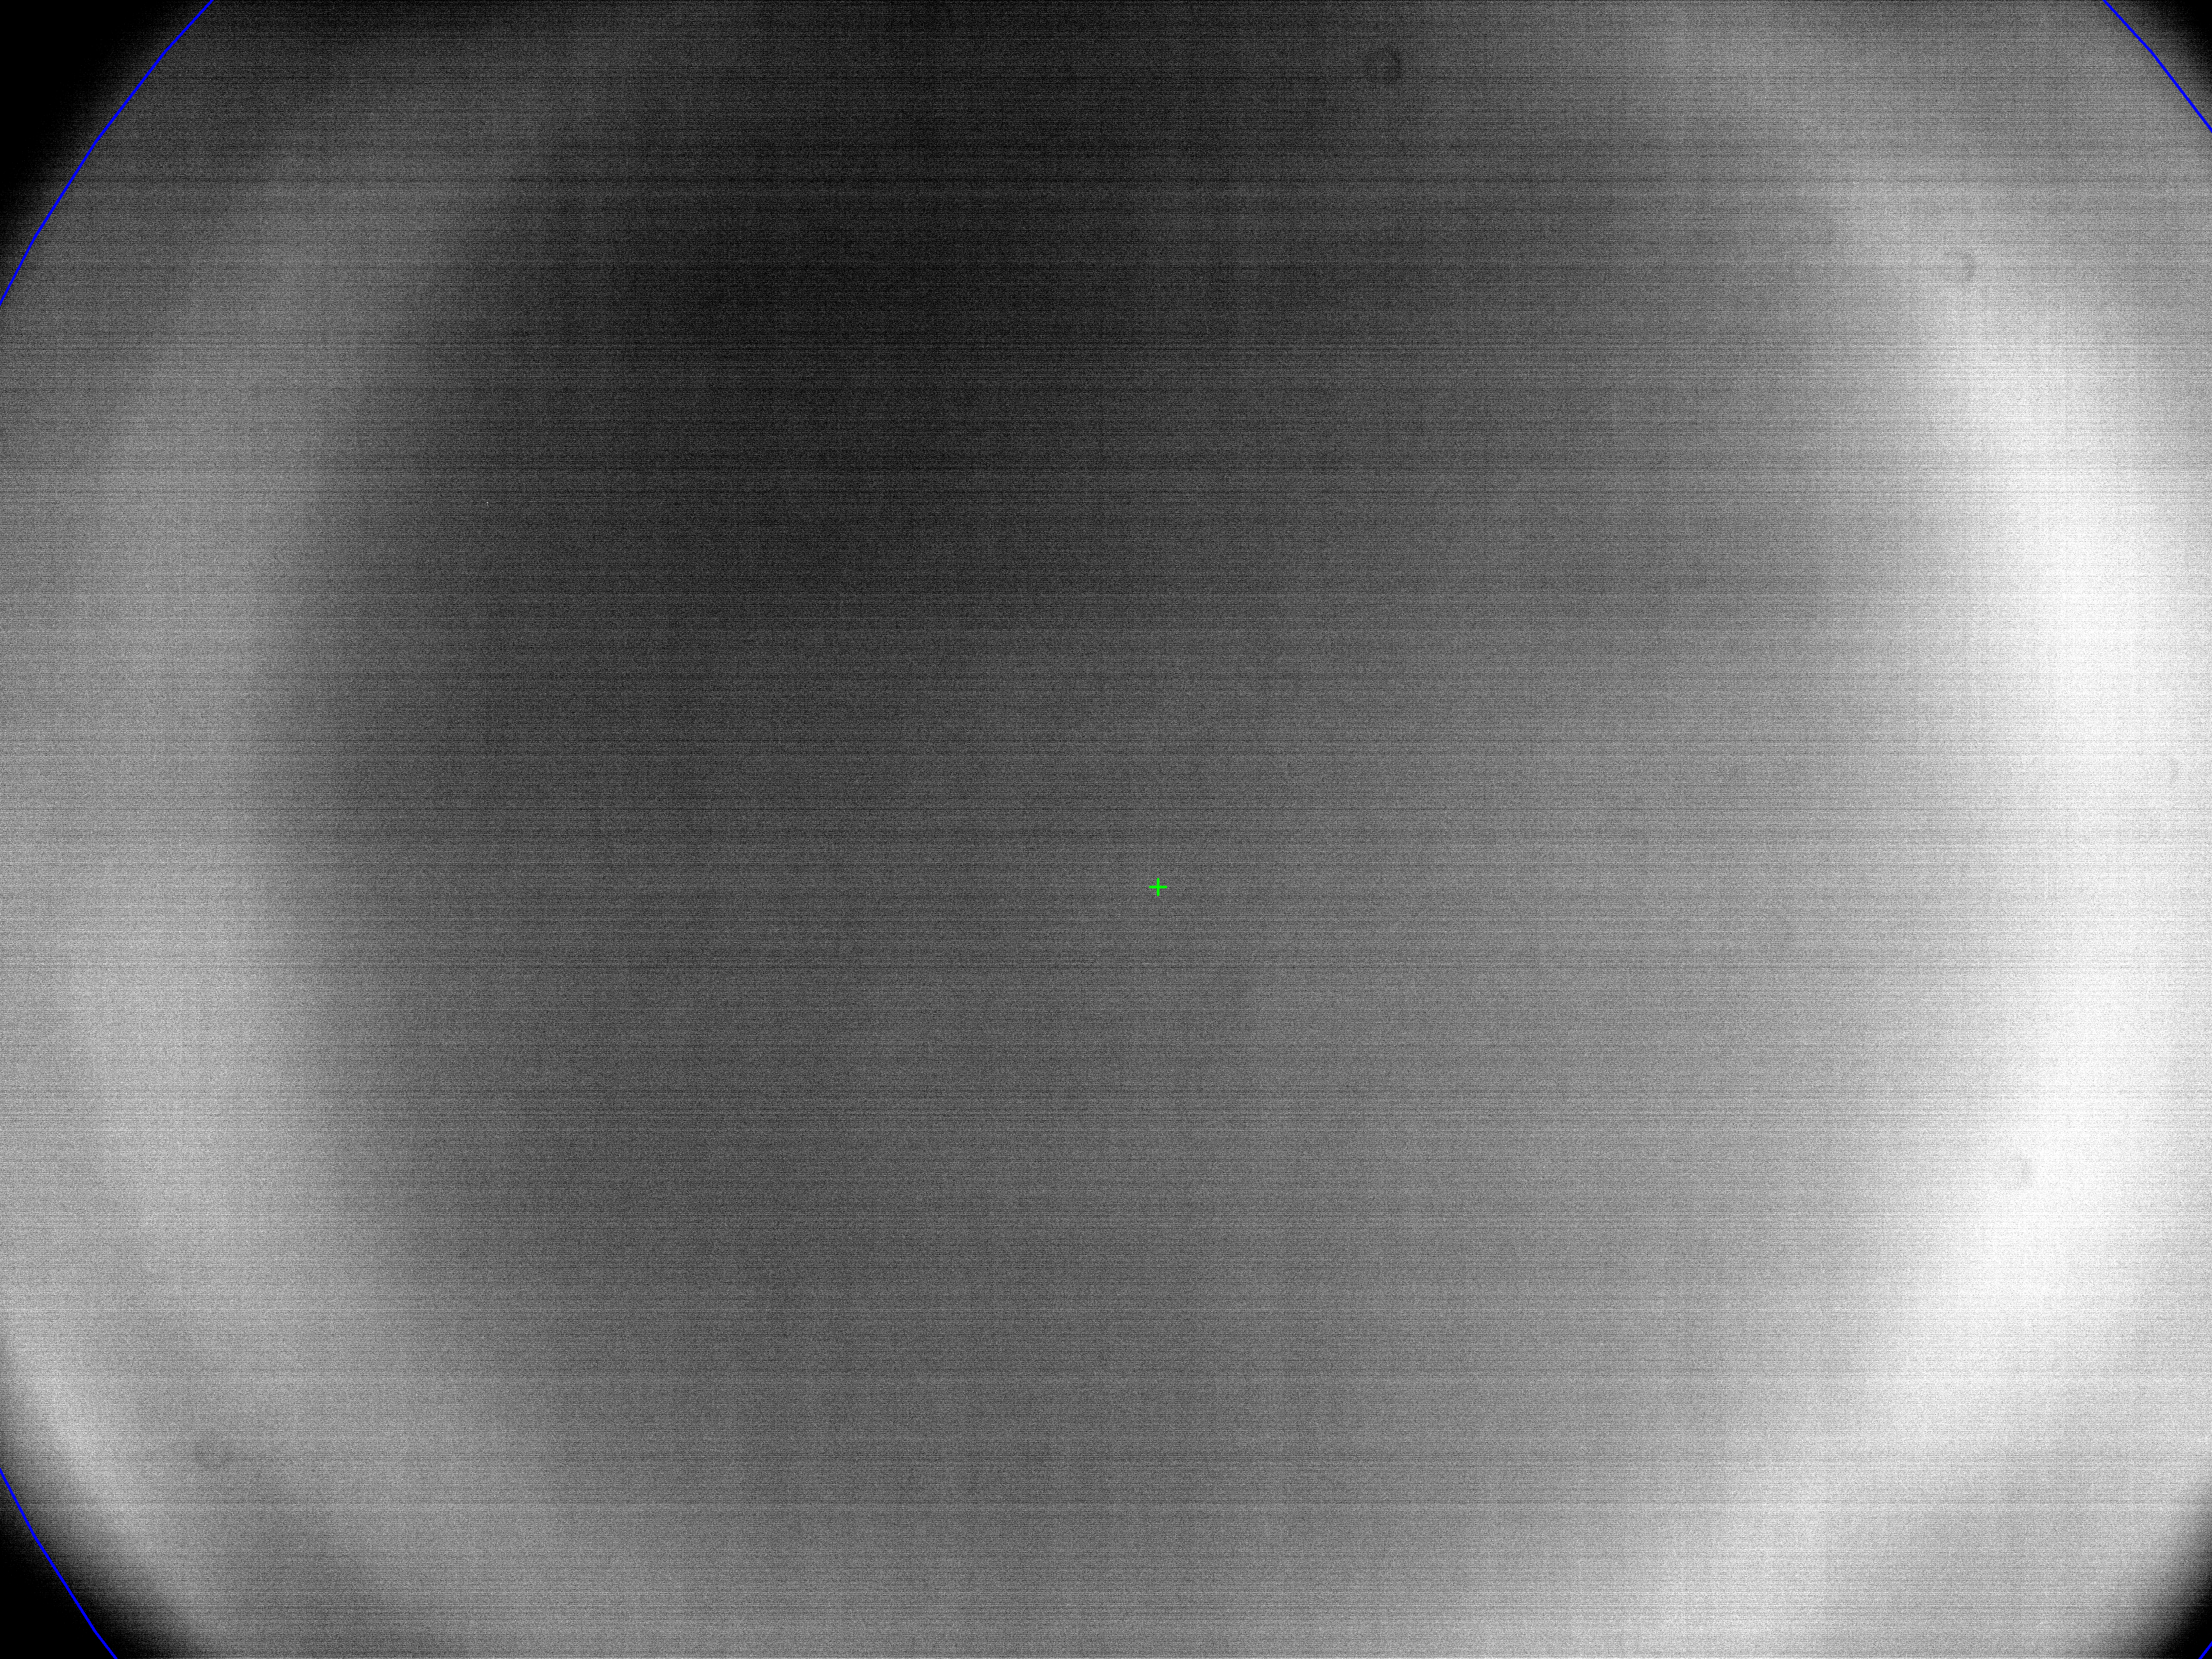
\includegraphics[width=0.75\linewidth]{Imagenes/flat_centro_optico.png}
    \caption{\small Ejemplo de flat con su ajuste de círculo dibujado en azul y el centro óptico en verde.}
    \label{fig:flat}
\end{figure}

Para dar una estimación del centro óptico se ha propone utilizar el \textit{Flat Frame}. Esto es una imagen de calibración utilizada en astrofotografía para corregir irregularidades ópticas como el viñeteo (esquinas oscuras), manchas de polvo en el sensor o filtro, y desalineaciones del campo. Se obtienen tomando una foto de una fuente de luz uniforme, permitiendo al software de procesado eliminar estos defectos. Debido a su simetría radial, es posible ajustar un círculo y usar el centro de este como centro óptico. En la Figura\ \ref{fig:flat} se puede observar un ejemplo de flat con su correspondiente ajuste y centro óptico marcado. Esto es simplemente una proposición y no se ha implementado en este caso concreto debido a la falta del flat. En cambio, se ha recurrido a la siguiente opción que es suponer como centro óptico el centro de la imagen que. Esta es una muy pobre aproximación y puede alterar notoriamente los resultados. Aunque, ante la falta de un flat se puede utilizar como opción de último recurso.\\

\begin{table}[ht]
\centering
\caption{\small Resultados medios obtenidos despúes de aplicar el método propuesto a imágenes proporcionadas por Satlantis Microsats.}
\label{tab:resultados_reales}
\begin{tabular}{ll}
\hline
\textbf{Parámetro} & \textbf{Valor} \\
\hline
Coeficiente de distorsión medido \(k_{\text{m}}\)  & \(29.2157\text{m}^{-2}\)\\
Error en el centro óptico \(\Delta C_o\)\ref{eq:error_centrooptico} &  - \\
MDLD & - \\
RMSE \(px\) & \(6.1427\times 10^{-6}\) \\
\(E_r\) & - \\
\(R^2\) & 0.7859 \\
\hline
\end{tabular}
\end{table}

Después de pasar las imágenes por el algortimo se han obtenido los resultados mostrados en la Tabla\ \ref{tab:resultados_reales}. La medida obtenida entra dentro del rango razonable que se esperaba: una distorsión de pocos píxeles a lo sumo. El error medio de los ajustes \(R^2\), no es bueno, pero es razonable y el RMSE es notoriamente bajo. El \(\Delta C_o\) no tiene mucho sentido en este caso; ya que, se ha partido de un \(C_o\) sin deamsiado rigor. El MDLD y el \(E_r\) no se pueden calcular; ya que, no se tienen los valores verdaderos.\\

En la Figura\ \ref{fig:maps_real} se muestra el mapa de distorsión y los ejes principales de la placa calculado por el algoritmo. Observando ambas figuras se puede intuir un pequeño error en el cálculo de la orientación; sobre todo, si nos fijamos en la silueta tipo "vórtice" del mapa de distorsión. Este peqeuño error ha podido empeorar la medida del coeficiente de distorisón. 

\begin{figure}[htbp]
    \centering
    \begin{minipage}{\textwidth}
        \centering
        % Subfigura 1
        \begin{subfigure}[t]{0.4\textwidth}
            \includegraphics[width=\linewidth]{Imagenes/img_RotMap_0000_real.png}
            \caption{\small Ejes principales calculados por el algoritmo en la imagen proporcionada por Satlantis Microsats.}
            \label{fig:rotmap_real}
        \end{subfigure}
        \hfill
        % Subfigura 2
        \begin{subfigure}[t]{0.4\textwidth}
            \includegraphics[width=\linewidth]{Imagenes/img_DistMap_0000_real.png}
            \caption{\small Mapa de distorsión calculado por el algoritmo en la imagen proporcionada por Satlantis Microsats. Las flechas (zoom x100) representan el desplazamiento de los pinholes \(M_i-P_i\). Los puntos rojo y verde son el centro de la placa y óptico respectivamente.}
            \label{fig:mapdist_real}
        \end{subfigure}
        \hfill
    \end{minipage}
    \caption{\small Representaciones asociadas a la imágenes proporcionadas por Satlantis Microsats}
    \label{fig:maps_real}
\end{figure}

\section{Conclusiones}
En este trabajo se ha propuesto un algortimo de detección de distorsión y se ha puesto en práctica con imágenes proporcionadas por Satlantis. Además, se han estudiado los límites y condiciones en los que la metodología poropuesta trabaja mejor y peor. Exitosamente se ha validado el algoritmo para calcular el perfil de distorsión de un único parametro que para cámaras profesionales es suficiente. El método, aún teniendo sus limitaciones y requerimientos como preparar el banco experimental (placa de pinholes, alineamiento de centro óptico, medidas del \(spacing\dots\)) se ha demostrado que es muy fiable. Para futuros trabajos se propone mejorar la modelización y alineamiento de los pinholes ideales.
\printbibliography
\end{document}
